\newpage
\epstopdfsetup{outdir=./}
\section{Simulation Analysis}
\label{sec:simulation}

\subsection{Operating Point Analysis for t $<$ 0}

The circuit was simulated and analysed using the Ngspice software. 

The results for step (1), which asked to simulate the operating point for t$<$0, are shown in the Table \ref{tab:op_sim1}.

\begin{table}[H]
  \centering
  \begin{tabular}{|l|r|}
    \hline    
    {\bf Name} & {\bf Value [A or V]} \\ \hline
    \input{../sim/op_tab}
  \end{tabular}
  \caption{Operating point for t$<$0. A variable preceded by @ is of type {\em current}
    and expressed in Ampere; other variables are of type {\it voltage} and expressed in
    Volt.}
  \label{tab:op_sim1}
\end{table}

By comparing this table with the one from the theoretical analysis, we can see slightly different values, which are probably caused by different approximations in Octave and Ngspice.

\subsection{Operating Point Analysis for t $=$ 0}

In step (2) the capacitor was replaced by a voltage source with the same voltages obtained in step (1) ($V_x = V_6 - V_8$) and $V_s$ was set to 0. The results are shown in the table.

\begin{table}[H]
  \centering
  \begin{tabular}{|l|r|}
    \hline    
    {\bf Name} & {\bf Value [A or V]} \\ \hline
    \input{../sim/op2_tab}
  \end{tabular}
  \caption{Operating point for t$=$0. A variable preceded by @ is of type {\em current}
    and expressed in Ampere; other variables are of type {\it voltage} and expressed in
    Volt.}
  \label{tab:op_sim2}
\end{table}

This step is needed to calculate the time constant.

\subsection{Natural solution for $V_6$ using transient analysis}

In step (3), the natural solution was simulated. The result of the transient analysis in the time interval [0s,20s] is shown in the graphic of the Figure \ref{fig:sim_natural}.

\begin{figure}[H] \centering
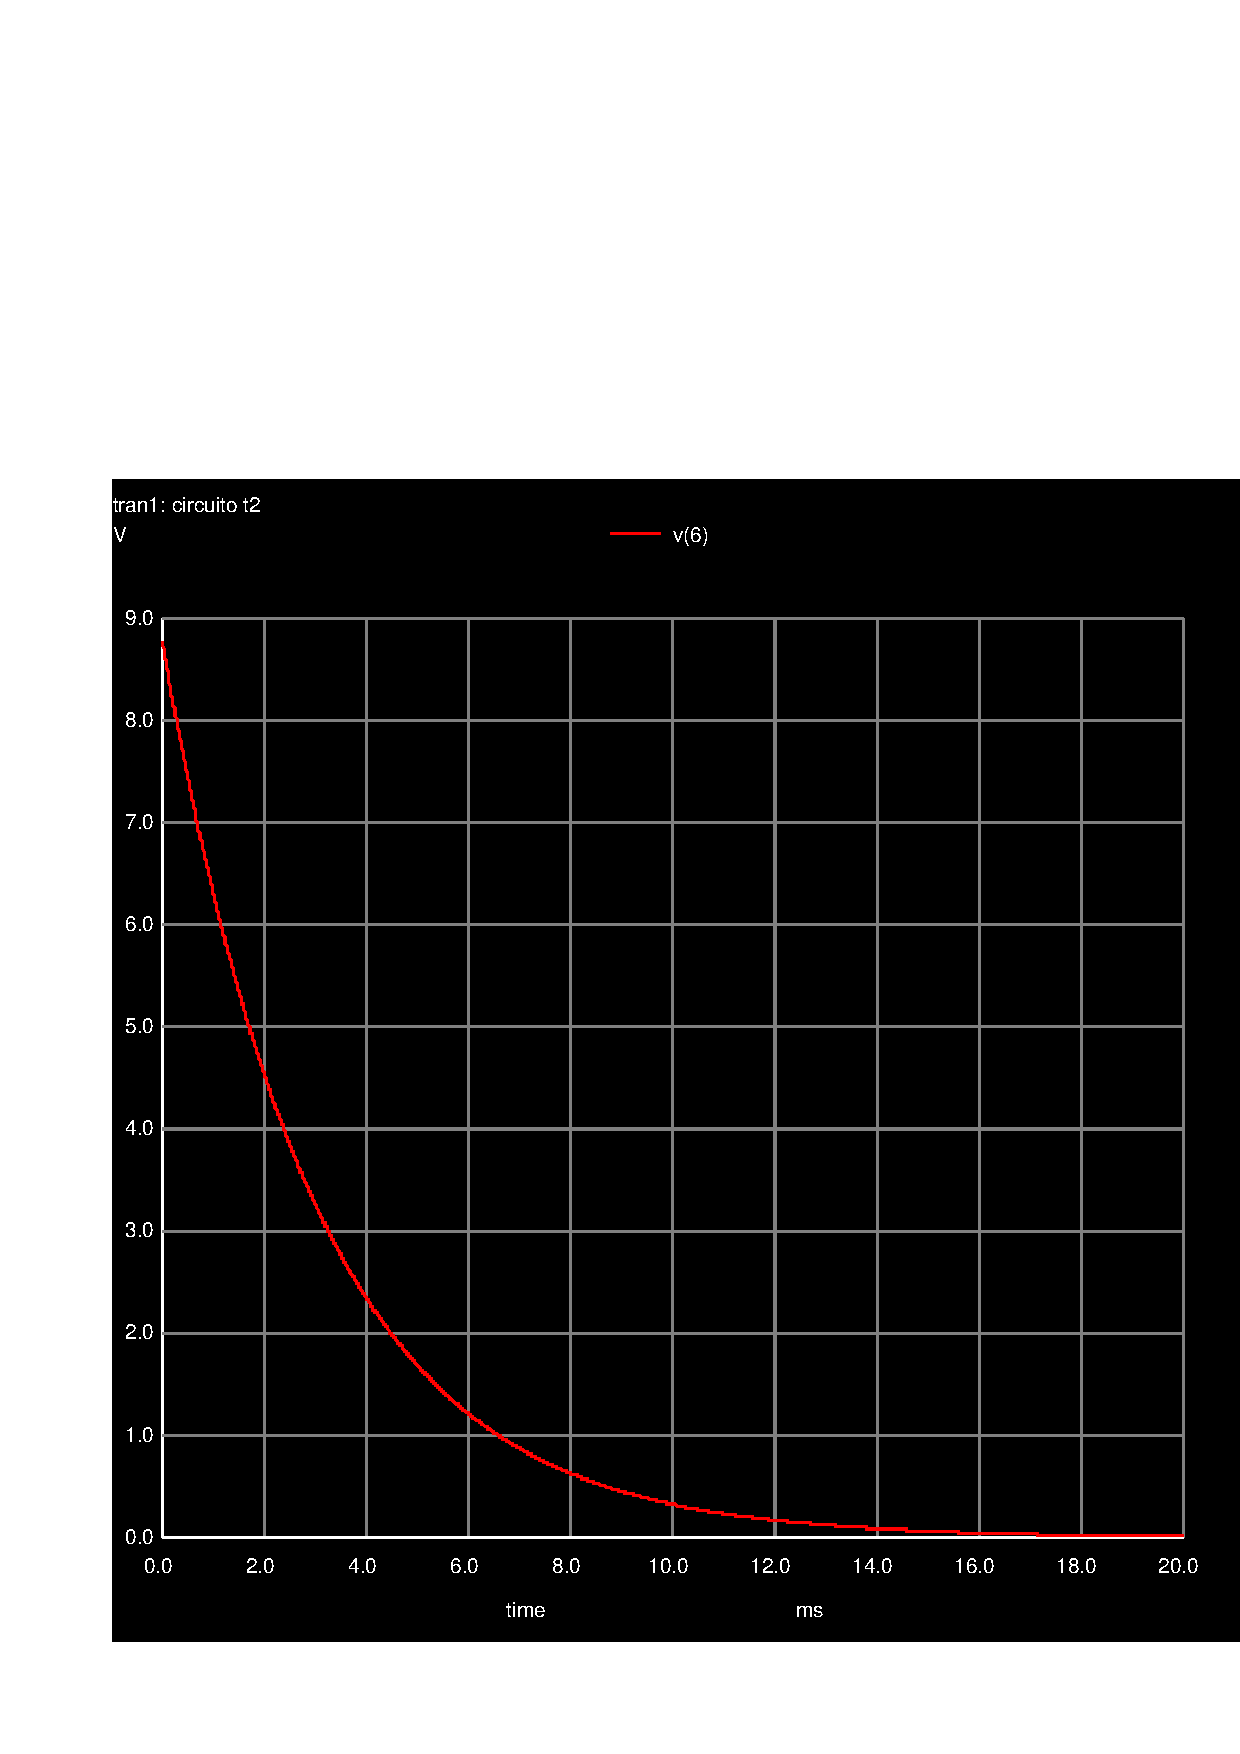
\includegraphics[width=0.8\linewidth]{trans.pdf}
\caption{Simulated natural response of $V_6(t)$ in the interval [0,20] ms. The \textit{x axis} represents the time in miliseconds and the \textit{y axis} the Potencial in node 6  in Volts.  }
\label{fig:sim_natural}
\end{figure}

Comparing to the graphic obtained with Octave, we can see there is no difference. 

\subsection{Total solution for $V_6$ using transient analysis}

Step (4) asked us to simulate the total (natural+forced) solution. For that, the frequency was given. We can see, in the graphic of the Figure \ref{fig:sim_total}, the stimulus and the response.

\begin{figure}[H] \centering
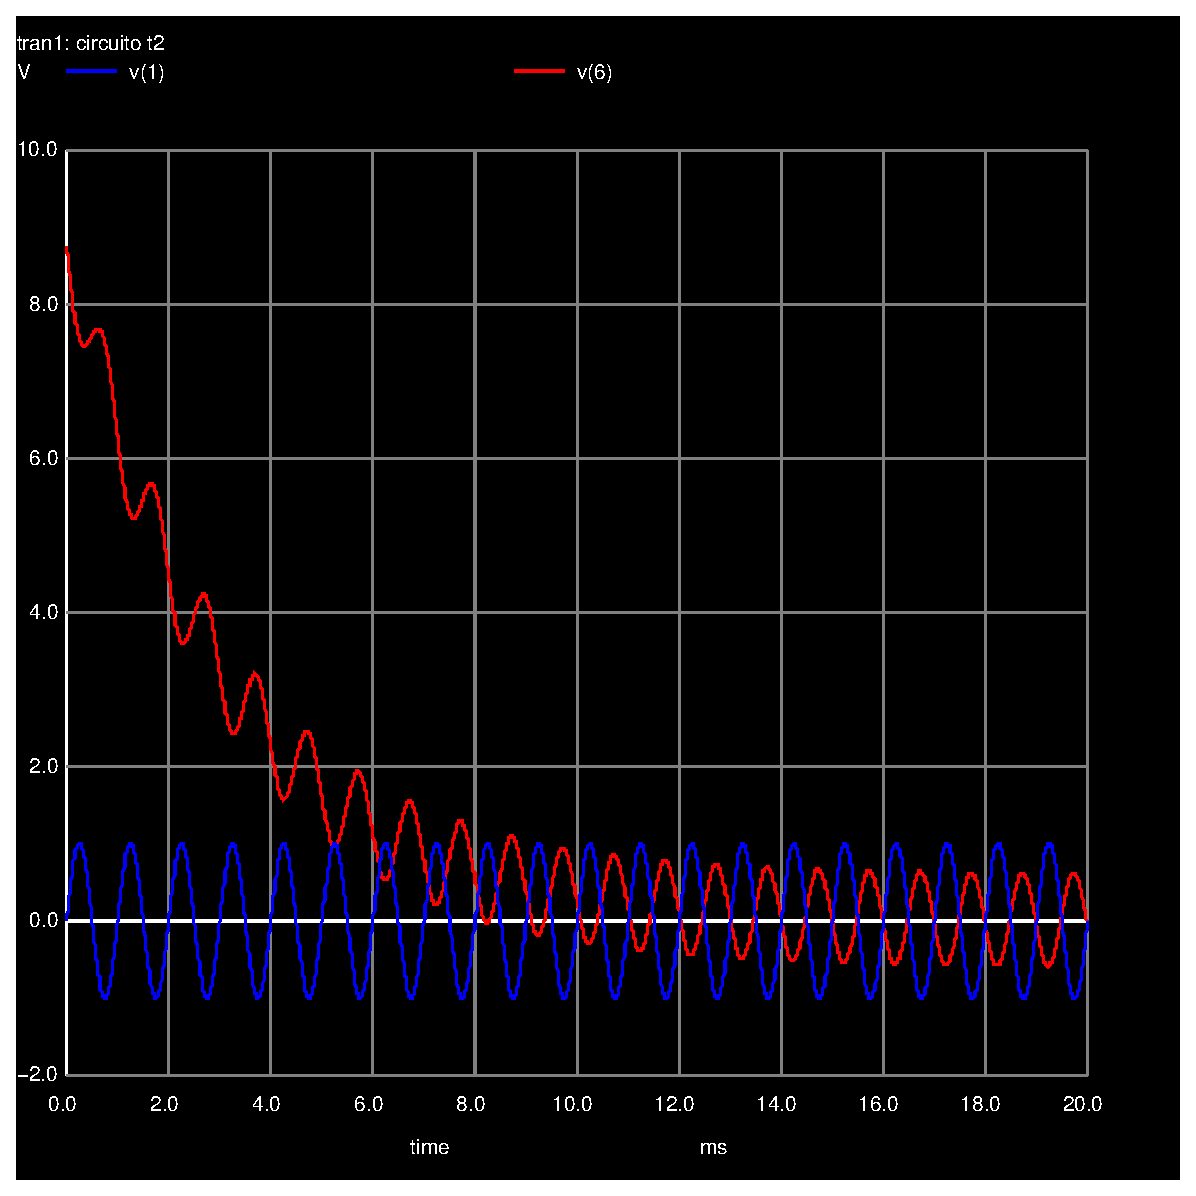
\includegraphics[width=0.8\linewidth]{trans4.eps}
\caption{Simulated total response of $V_6(t)$ in the interval [0,20] ms. The \textit{x axis} represents the time in miliseconds and the \textit{y axis} the Potencial in node 6  in Volts.  }
\label{fig:sim_total}
\end{figure}

Once again, the graphic obtained in Octave is the same.

\subsection{Frequency response in node 6}

Finally, in step (5), it was asked to simulate the frequency response between 0.1 Hz and 1 MHz.In the following Figures \ref{fig:sim_acm} and \ref{fig:sim_phase}, the amplitude frequency response and the phase response were plotted. It is important to notice that the frequency logscale has its magnitude in dB units and the phase is presented in degrees.


\begin{figure}[H] \centering
\includegraphics[width=0.8\linewidth]{acm.pdf}
\caption{Amplitude frequency response for $v_s(f)$, $v_6(f)$ and $v_c(f)$ in the interval [0.1, 1M]Hz. The $x$ axis has the frequency in Hz (logarithmic scale) and the $y$ axis has the amplitude in dB. }
\label{fig:sim_acm}
\end{figure}
\par
\begin{figure}[H] \centering
\includegraphics[width=0.8\linewidth]{phase.pdf}
\caption{Phase response for $v_s(f)$, $v_6(f)$ and $v_c(f)$ in the interval [0.1, 1M]Hz. The $x$ axis has the frequency in Hz (logarithmic scale) and the $y$ axis has the amplitude in dB.}
\label{fig:sim_phase}
\end{figure}



